%%
%  ******************************************************************************
%  * #file    Szablon_raportu_EN_Latex.tex
%  * #author  Adrian Wójcik   adrian.wojcik(at)put.poznan.pl
%  *          
%  * #commit  Patryk Kościk   koscikpatryk(at)gmail.com
%  *          Modified the template for Projekt przejsciowy purposes          
%  *          
%  *
%  * #commit  Patryk Kościk   koscikpatryk(at)gmail.com
%  *          Zupełnie przewrócono na łeb formatke po taktycznym wyjasnieniu          
%  *          
%  * #version 1.1
%  * #date    09-Mar-2022
%  * #brief   PROJPRZEJ
%  *
%  ******************************************************************************
%%  
\documentclass[11pt, a4paper]{article}

\usepackage{SM_template}

% Wypełnijcie te dyrektywy zgodnie z waszym tematem
%
% \lab      -> NAZWA CZUJNIKA,          np.: 'DHT22'
% \comment  -> Króciutki opis co to,    np.: 'Cyfrowy czujnik temperatury'
% \author   -> Autor dokumentu          np.: Patryk Kościk
%
% Pamiętajcie o zmianie ścieżki w \addbibresourcue (!)

\lab{Moduł KY-005 i HW-477}
\comment{Nadajnik i odbiornik promieniowania podczerwonego}
\author{Jakub Grzesiak}
\addbibresource{bib/HW-477.bib}

%
% Początek dokumentu
%
\begin{document}

%
% Strona tytułowa
%
\mainpage{HW-477/zdj_modułu/hw_477_gimp.jpg}
\newpage

\section*{Opis elementu}
Nadajnik promieniowania podczerwonego (ang. infrared transmitter) to moduł wyjściowy emitujący światło podczerwone IR o częstotliwości 38 kHz. Moduł w większości zastosowań wysyła dane poprzez promieniowanie wytwarzane przez diodę IR do odbiornika podczerwieni (ang. infrared receiver). Moduły te znajdują zastosowanie w takich urządzeniach jak: piloty do zdalnego sterowania urządzeniami elektronicznymi, np. telewizorami, oświetleniem czy klimatyzacją.
Nadajnik wraz z wyprowadzeniami przedstawiono na rysunku (\ref{fig:_transmitter_pinout}) a odbiornik na rysunku (\ref{fig:_receiver_pinout}).


%%%%%%%%%%%%%%%%%%%%%%%%%  TWO IMAGES SIDE BY SIDE  %%%%%%%%%%%%%%%%%%%%%%%%%%%%%
\vspace{0.25cm}
\begin{figure}[h]
\centering
%%%%%%%%%%%%%%%%%%%%%%%%%%%%%%%%%%%%%%%%%%%%%%%%%%%%%%%%%%%%%%%%%%%%%%%%%%%%%%%%%
\begin{subfigure}{.5\textwidth}
\centering
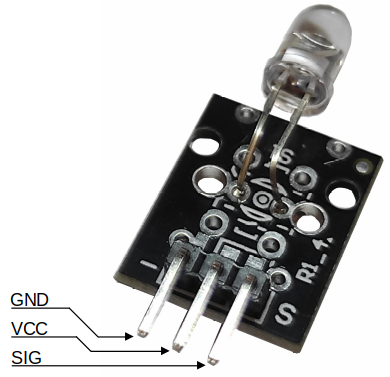
\includegraphics[width=0.65\linewidth]{fig/HW-477/zdj_modułu/transmitter_pinout.png}
\caption{Fizyczna budowa nadajnika wraz z pinoutem}
\label{fig:_transmitter_pinout}
\end{subfigure}%
%%%%%%%%%%%%%%%%%%%%%%%%%%%%%%%%%%%%%%%%%%%%%%%%%%%%%%%%%%%%%%%%%%%%%%%%%%%%%%%%%
\begin{subfigure}{.5\textwidth}
\centering
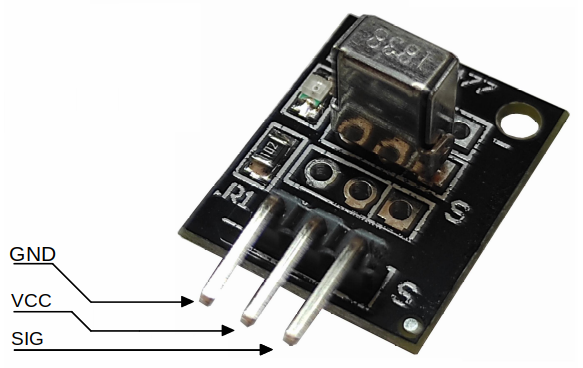
\includegraphics[width=0.99\linewidth]{fig/HW-477/zdj_modułu/receiver_pinout.png}
\caption{Fizyczna budowa odbiornika wraz z pinoutem}
\label{fig:_receiver_pinout}
\end{subfigure}
%%%%%%%%%%%%%%%%%%%%%%%%%%%%%%%%%%%%%%%%%%%%%%%%%%%%%%%%%%%%%%%%%%%%%%%%%%%%%%%%%
% \caption{PODPIS}
\label{fig:element}
\end{figure}
\vspace{0.25cm}
%%%%%%%%%%%%%%%%%%%%%%%%%  TWO IMAGES SIDE BY SIDE  %%%%%%%%%%%%%%%%%%%%%%%%%%%%%

% \subsection{Opis modułu} REPLACE SUBSECTION WITH 1CM VSPACE
Moduł nadajnika może być zasilanyn napięciem $5V DC$ a moduł odbiornika napięciami z zakresu $2,7V - 5,5V DC$.
Schematy budowy wewnętrznej nadajnika i odbiornika przedstawiono poniżej. Rezystor R1 na schemacie odbiornika jest odpowiedzialny za ograniczenie prądu diody sygnalizacyjnej.


%%%%%%%%%%%%%%%%%%%%%%%%%  TWO IMAGES SIDE BY SIDE  %%%%%%%%%%%%%%%%%%%%%%%%%%%%%
\begin{figure}[h]
\centering
%%%%%%%%%%%%%%%%%%%%%%%%%%%%%%%%%%%%%%%%%%%%%%%%%%%%%%%%%%%%%%%%%%%%%%%%%%%%%%%%%
\begin{subfigure}{.5\textwidth}
\centering
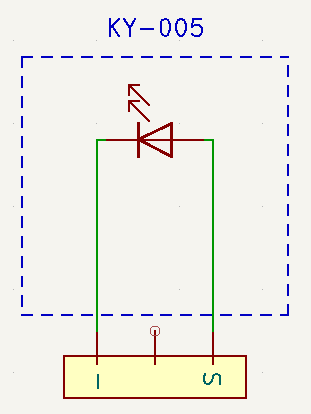
\includegraphics[width=.63\linewidth]{fig/HW-477/zdj_modułu/transmitter_scheme.png}
\caption{Schemat budowy wewnętrznej nadajnika}
\label{fig:_schemat_nadajnik}
\end{subfigure}%
%%%%%%%%%%%%%%%%%%%%%%%%%%%%%%%%%%%%%%%%%%%%%%%%%%%%%%%%%%%%%%%%%%%%%%%%%%%%%%%%%
\begin{subfigure}{.5\textwidth}
\centering
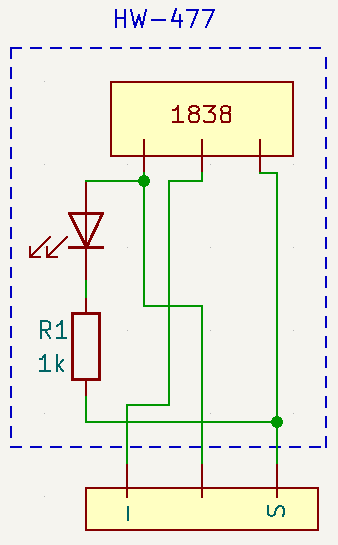
\includegraphics[width=.51\linewidth]{fig/HW-477/zdj_modułu/receiver_scheme.png}
\caption{Schemat budowy wewnętrznej odbiornika}
\label{fig:_schemat_odbiornik}
\end{subfigure}
%%%%%%%%%%%%%%%%%%%%%%%%%%%%%%%%%%%%%%%%%%%%%%%%%%%%%%%%%%%%%%%%%%%%%%%%%%%%%%%%%
\label{fig:modul}
\end{figure}
\vspace{0.25cm}
%%%%%%%%%%%%%%%%%%%%%%%%%  TWO IMAGES SIDE BY SIDE  %%%%%%%%%%%%%%%%%%%%%%%%%%%%%
Działanie układu złożonego z nadajnika i odbiornika polega na przesyłaniu ramek danych binarnych złożonych z ciągu impulsów podczerwieni do odbiornika. Wielu producentów (np. Sharp, LG, Apple, Sony i inni) stworzyło własne protokoły przesyłu danych przez podczerwień. Protokoły różnią się głównie częstotliwością przenoszenia i długością trwania impulsów - modulacja szerokości impulsów. Nadawanie i dekodowanie danych realizowane jest przez program zaimplementowany na mikroprocesorze.


\newpage

\section{Użycie czujnika}
Oba moduły posiadają 3 wyprowadzenia - dwa zasilające i jedno sygnałowe. Działanie modułów można zweryfikować przy użyciu dwóch mikrokontrolerów - jednego z podłączonym nadajnikiem, a drugiego z odbiornikiem. W poniższym przykładzie użyto płytki Arduino UNO - pozwala to na użycie biblioteki "IRremote", która implementuje wiele standardów protokołów do przesyłu i odbioru danych przez podczerwień. Układ połączeń został przedstawiony na rysunku (\ref{fig:_polaczenie_ukladu}). Należy pamiętać, aby podłączyć pin sygnałowy 'S' nadajnika do portu skonfigurowanego w mikroprocesorze jako wyjście, a pin signałowy 'S' odbiornika do portu wejściowego mikroprocesora.

\vspace{0.25cm}
\begin{figure}[h]
    \centering
    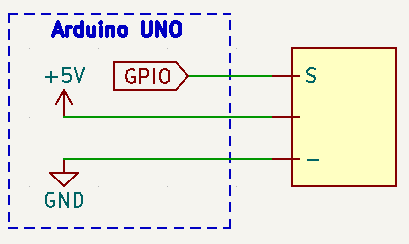
\includegraphics[width=0.6\textwidth]{fig/HW-477/polaczenie_modulu/adruino_con.png}
    \caption{Połączenie układu z mikroprocesorem}
    \label{fig:_polaczenie_ukladu}
\end{figure}
\vspace{0.25cm}

Poniżej zaprezentowano zdjęcia rzeczywistego układu. Kod zaimplementowany na mikroprocesorze zawarty jest w \texttt{Suplement \#1}.

% TUTAJ FOTY ODNOSNIE TEGO
%%%%%%%%%%%%%%%%%%%%%%%%%  TWO IMAGES SIDE BY SIDE  %%%%%%%%%%%%%%%%%%%%%%%%%%%%%
\vspace{0.25cm}
\begin{figure}[h]
\centering
%%%%%%%%%%%%%%%%%%%%%%%%%%%%%%%%%%%%%%%%%%%%%%%%%%%%%%%%%%%%%%%%%%%%%%%%%%%%%%%%%
\begin{subfigure}{.5\textwidth}
\centering
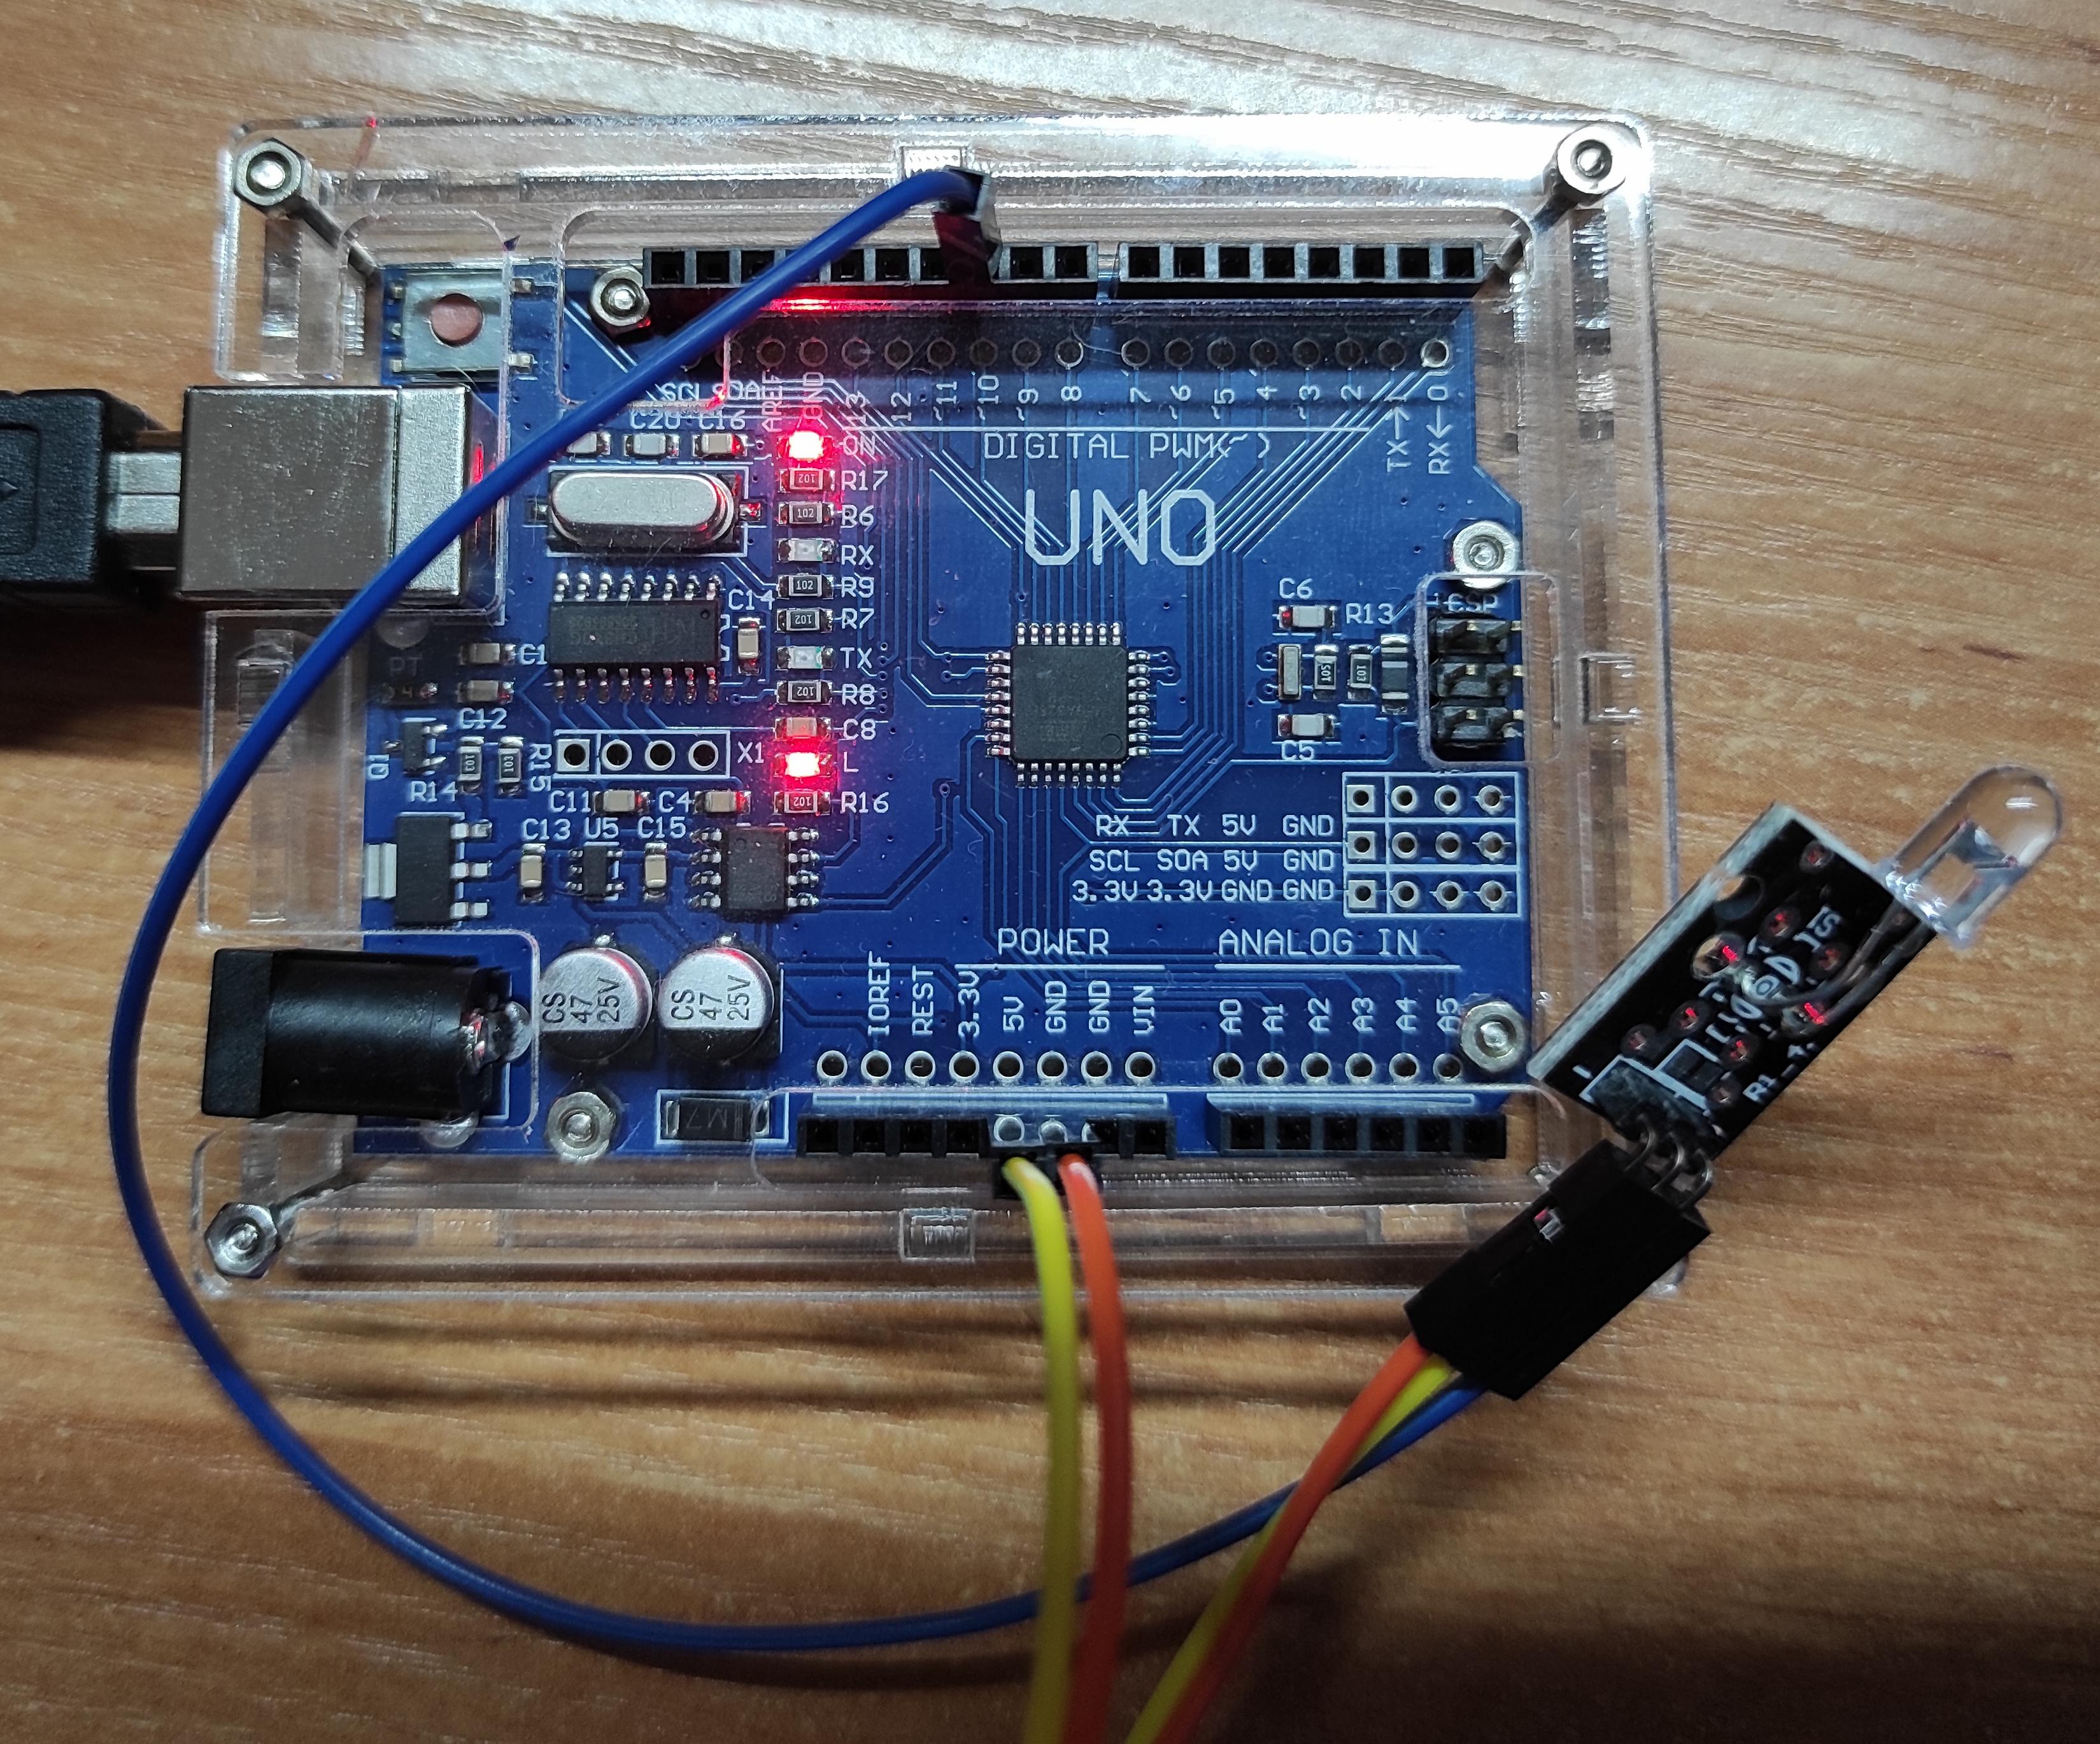
\includegraphics[width=.8\linewidth]{fig/HW-477/działanie_ukladu/transmitter_uno.jpg}
\caption{Połączenie nadajnika z mikroprocesorem}
\label{fig:_uklad_off}
\end{subfigure}%
%%%%%%%%%%%%%%%%%%%%%%%%%%%%%%%%%%%%%%%%%%%%%%%%%%%%%%%%%%%%%%%%%%%%%%%%%%%%%%%%%
\begin{subfigure}{.5\textwidth}
\centering
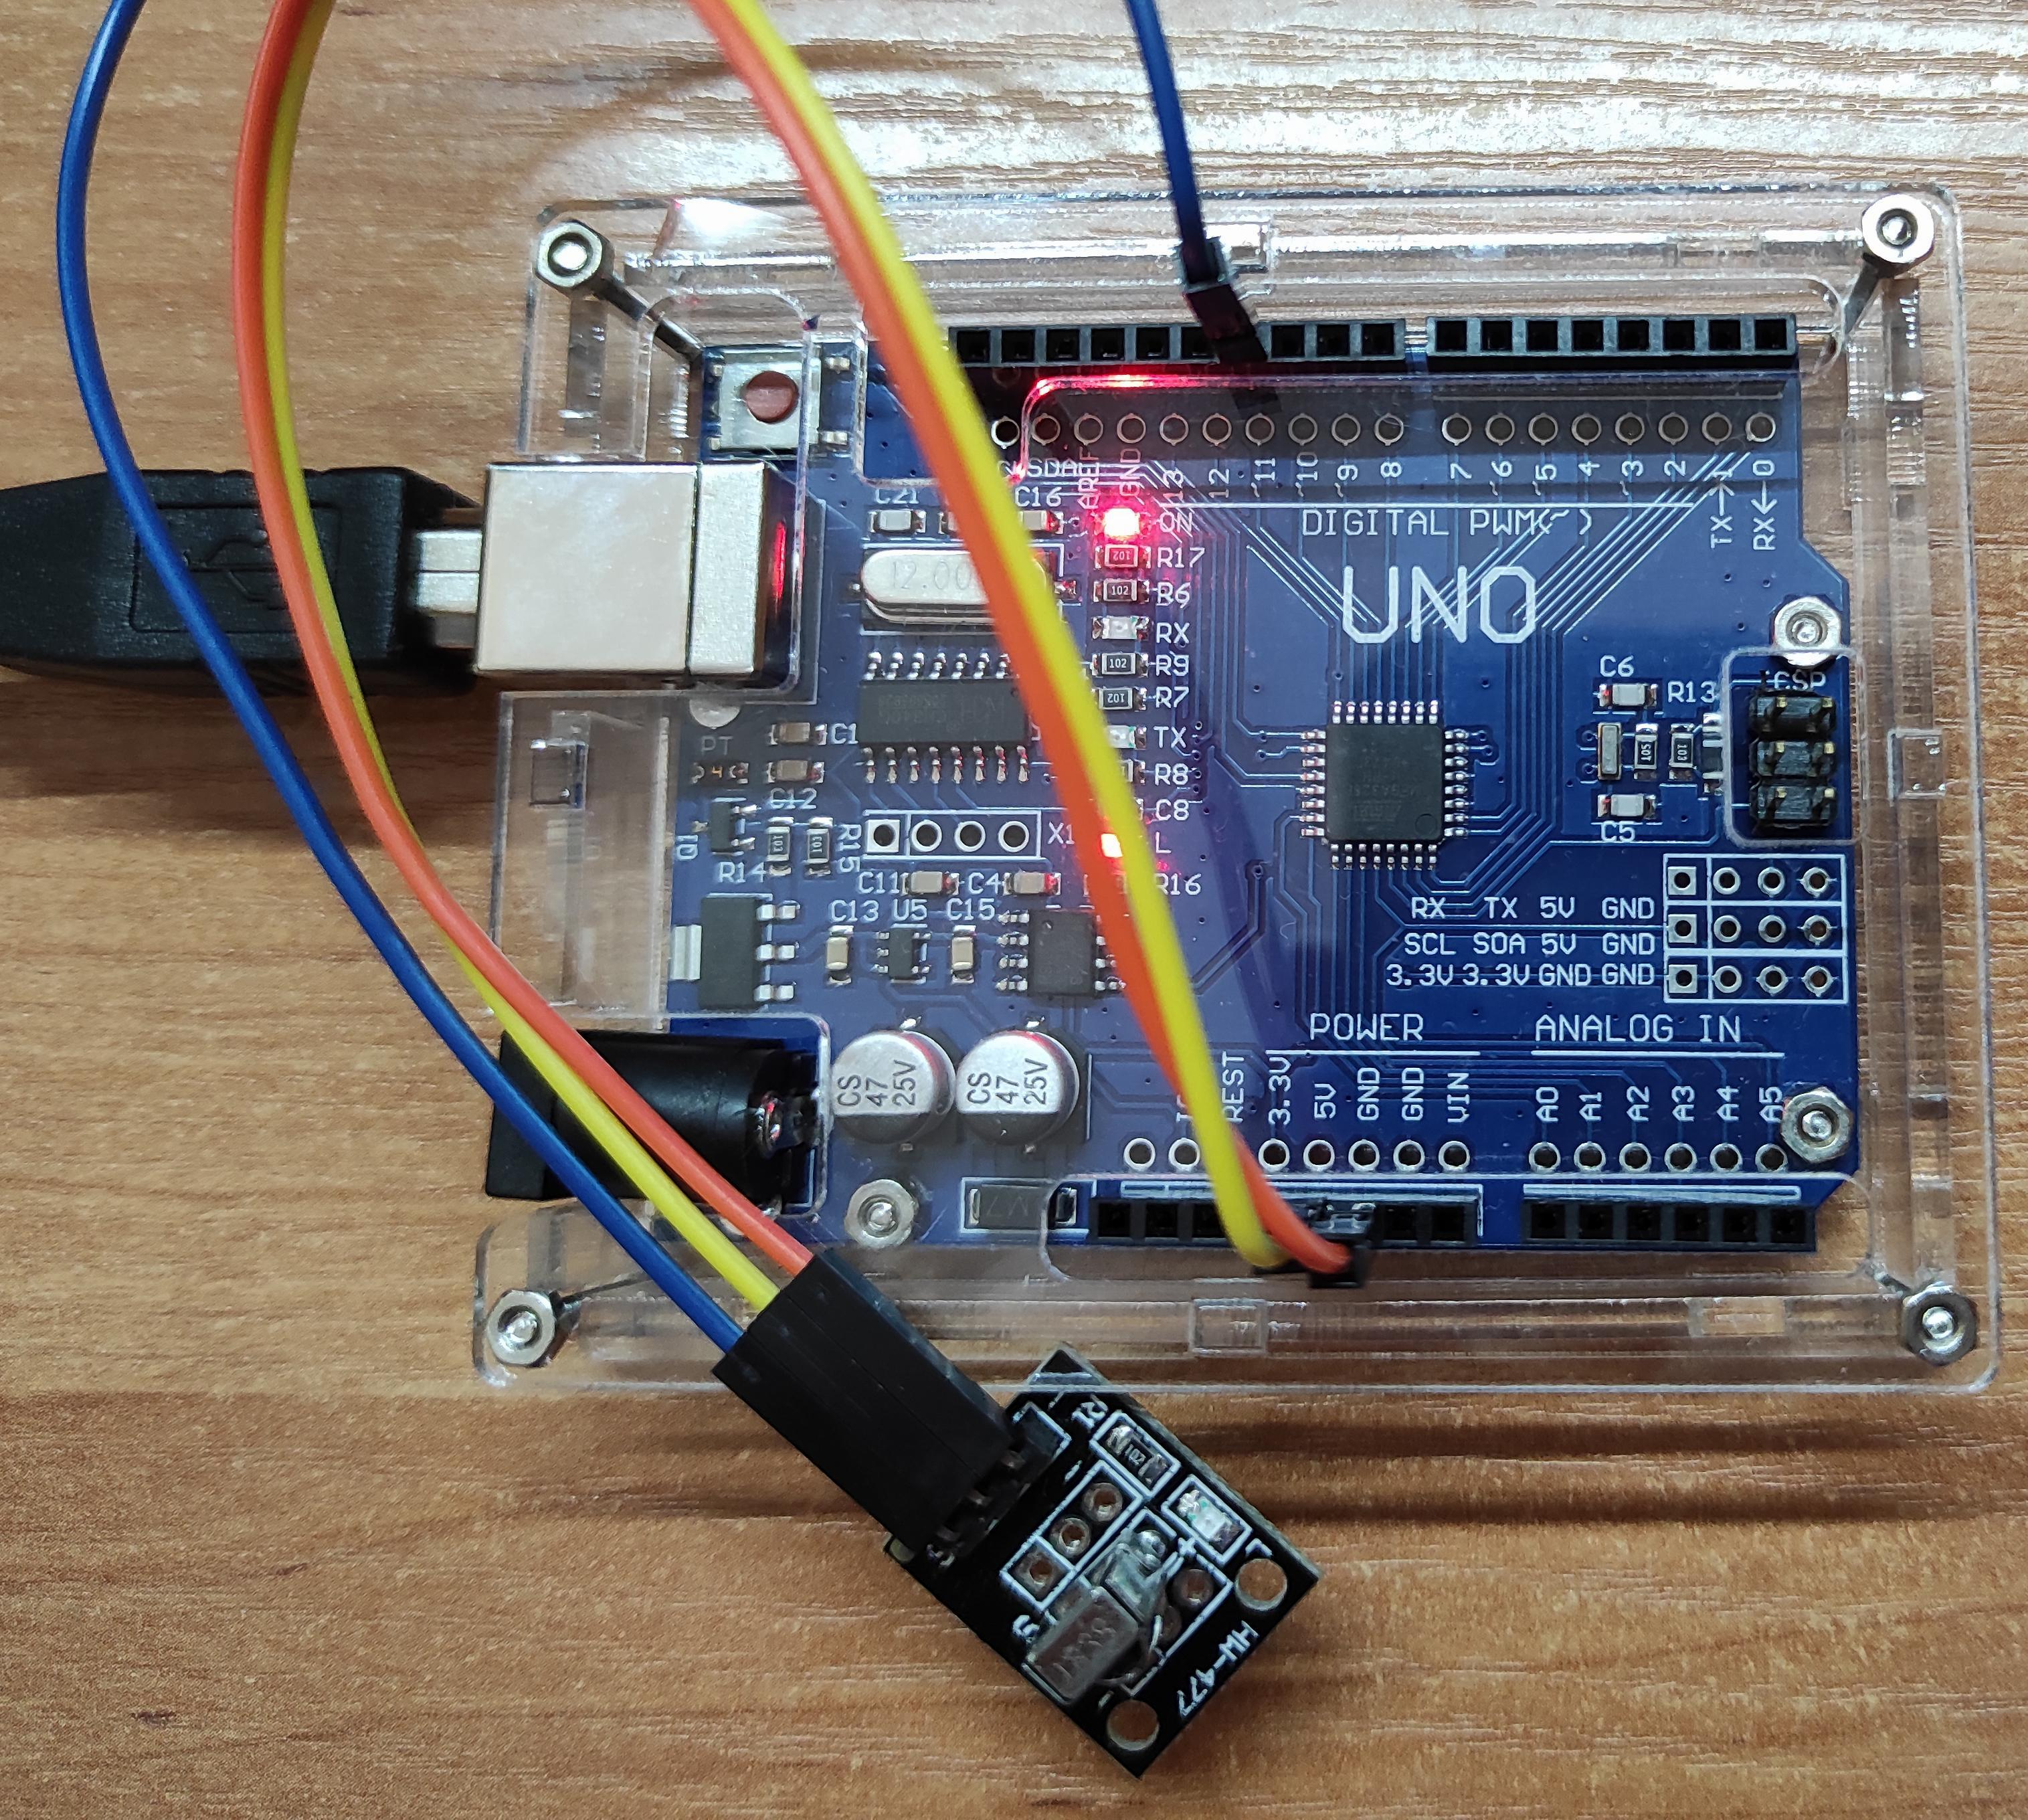
\includegraphics[width=.74\linewidth]{fig/HW-477/działanie_ukladu/receiver_uno.jpg}
\caption{Połączenie odbiornika z mikroprocesorem}
\label{fig:_uklad_on}
\end{subfigure}
%%%%%%%%%%%%%%%%%%%%%%%%%%%%%%%%%%%%%%%%%%%%%%%%%%%%%%%%%%%%%%%%%%%%%%%%%%%%%%%%%
% \caption{PODPIS}
\label{fig:mikroproc}
\end{figure}
\vspace{0.25cm}
%%%%%%%%%%%%%%%%%%%%%%%%%  TWO IMAGES SIDE BY SIDE  %%%%%%%%%%%%%%%%%%%%%%%%%%%%%

\vspace{0.25cm}
\begin{figure}[h]
    \centering
    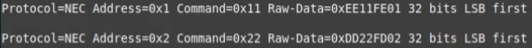
\includegraphics[width=0.6\textwidth]{fig/HW-477/działanie_ukladu/serial_port.png}
    \caption{Przykładowy odczyt wysłanych danych}
    \label{fig:_serial}
\end{figure}
\vspace{0.25cm}


Dodatkowo działanie układu przedstawiono na załączonym w \texttt{Suplement Wideo} materiale 
wideo.

\newpage
\printbibliography[heading=bibintoc]

\end{document}